
\chapter{Análisis}

En este capítulo se describe la fase de análisis del problema a tratar. En concreto desarrollo la descripción de los implicados en el proceso y la especificación de requisitos funcionales, no funcionales y de información que debe cubrir la solución al problema. Como refuerzo para los requisitos del proyecto, se incluyen diagramas de casos de uso en los que interviene cada uno de los implicados.\newline

\section{Descripción de los implicados} \label{implicados}

En esta aplicación, destacamos dos principales implicados: el administrador de la aplicación y el usuario final de la aplicación.

\begin{itemize}
	\item \textbf{Desarrollador y administrador del sistema}: La responsabilidad del implicado será la de realizar las distintas actividades de desarrollo de la aplicación: corregir errores o añadir nuevas features, entre otras actualizaciones, que garantizan el correcto funcionamiento del sistema y su mantenimiento. Se encargará también de las tareas de gestión de la base de datos como puede ser añadir nuevos usuarios.
	
	\item \textbf{Usuario de la aplicación}: Este implicado representa al cliente que usa la aplicación. Este implicado hace uso de la aplicación como usuario final.
\end{itemize}

\section{Especificación de requisitos}

\subsection{Requisitos Funcionales}

Descripción de los requisitos más importantes a nivel de funciones que debe incluir el sistema, realizando una clasificación en categorías, a cada uno de los requisitos se le ha asignado un código y un nombre, con el fin de identificarlos fácilmente a lo largo de todo el proyecto. 

\begin{itemize}
	
	\item \textbf{RF-1. Iniciar sesión en la aplicación.} El usuario de la aplicación deberá iniciar sesión en la APP para hacer uso de la misma. El sistema por tanto incluirá un \textbf{sistema de gestión de usuarios}.
	
	\item \textbf{RF-2. Gestiones de la plataforma de trading.} 
	\begin{itemize}
		\item \textbf{RF-2.1. Login en la plataforma de trading.} El usuario de la aplicación podrá conectarse con su cuenta de trading, comercial o demo, para poder hacer el uso completo de la APP.
		\item \textbf{RF-2.2. Ver capital disponible.} El usuario podrá ver el capital disponible en su cuenta de trading.
		\item \textbf{RF-2.3. El usuario podrá ver información de las operaciones} realizadas y de operaciones que en ese momento aún no se han cerrado.
	\end{itemize}

	\item \textbf{RF-3. Gestión de datos.} El usuario de la aplicación podrá elegir qué datos descargar y guardar en la base de datos. Estos datos históricos comenzarán desde cualquier fecha disponible hasta la actualidad. Los datos pertenecerán a un mercado financiero específico y tendrán una temporalidad específica, siguiendo el formato \textit{OHLC}.

	\item \textbf{RF-4. Visualización de datos.} El usuario de la aplicación podrá ver información de precios de un mercado financiero específico.
	\begin{itemize}
		\item \textbf{RF-4.1. Ver datos de mercado en rango de tiempo específico.} El usuario de la aplicación podrá ver información de precios entre dos fechas específicas.
		\item \textbf{RF-4.2. Ver datos de mercado con un marco de tiempo específico en tiempo real.} El usuario de la aplicación podrá ver información de precios en tiempo real con un marco de tiempo específico.
	\end{itemize}

	\item \textbf{RF-5. El usuario podrá elegir un modelo y realizar trading algorítmico.} También podrá parametrizarlo según modelo y elegir tiempo en el que quiere dejar haciendo las operaciones automáticas. 

	\item \textbf{RF-6. El usuario podrá elegir un modelo y realizar trading algorítmico a modo de backtesting.} De esta forma podrá probar cada uno de los modelos en un mercado y periodo de tiempo prefijados.
	
\end{itemize}

\subsection{Requisitos No Funcionales}

\begin{itemize}
	\item \textbf{RNF-1}. La plataforma de trading que usará la aplicación será \textit{MetaTrader5}.
	\item \textbf{RNF-2}. La aplicación permitirá el uso de cualquier bróker aceptado por \textit{MetaTrader5}.
	\item \textbf{RNF-3}. Para la visualización de datos, el usuario podrá elegir un marco de tiempo de entre m1, m3, m5, m15, m30 ó m45; h1, h2, h3 ó h4; d1 (minutos, horas o días, respectivamente).
	\item \textbf{RNF-4}. La aplicación responderá a las peticiones de los usuarios en un tiempo determinado,
	mostrando un aviso de error si el tiempo de respuesta es superior al establecido.
	\item \textbf{RNF-5}. La aplicación deberá funcionar computadoras mediante navegador web.
	\item \textbf{RNF-6}. Para la implementación de la aplicación, se utilizará \textit{Python} y su framework \textit{Django}.
	\item \textbf{RNF-7}. La interfaz debe ser sencilla e intuitiva.
\end{itemize}

\subsection{Requisitos de Información}

\begin{itemize}
	\item \textbf{RI-1}. El sistema gestor de bases de datos utilizado será \textit{SQLite3}.
\end{itemize}

\section{Diagramas de casos de uso}

En esta sección, muestro los distintos diagramas de cada caso de uso que implementa la aplicación. Con estos diagramas se completa la fase de análisis del proyecto y con ellos vemos los roles que tienen los implicados y cómo interactúan con el sistema. Véase punto \ref{implicados}, descripción de actores o implicados.

\subsection{Gestión de sesiones de la APP}

En el diagrama \ref{cu1} se representan los casos de uso referentes al sistema de gestión de usuarios de la aplicación. \newline

El usuario de la aplicación deberá identificarse y cerrar sesión en \textit{TradingAPP}. Estas acciones de Login y Logout interactúan internamente con el módulo de \textit{Django}, que es el que implementa el sistema de sesiones. \newline

A su vez, el administrador de la APP será quién administre los usuarios, a través del módulo de \textit{Django}. 

\begin{figure}[h] 
	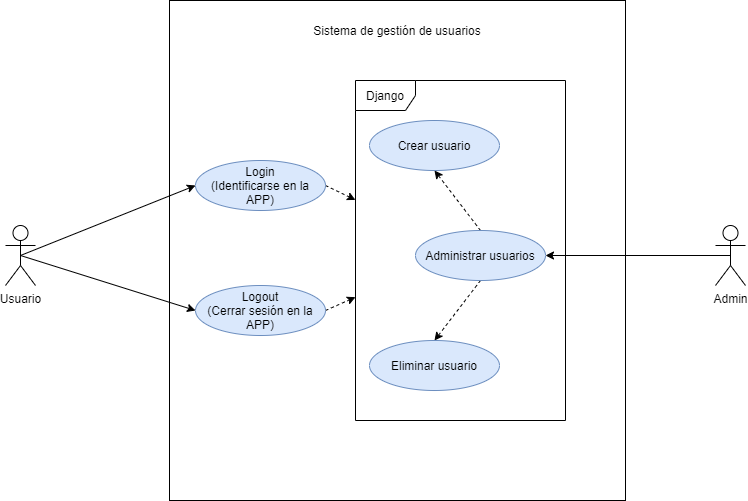
\includegraphics[width=1\textwidth]{imagenes/diagramas_casos_de_uso/CU1-gestion_usuarios.png} 
	\caption{Diagrama de casos de uso referente al sistema de gestión de usuarios de la APP} \label{cu1}
\end{figure}

\subsection{Gestiones de la plataforma de trading (MT5)}

En el diagrama \ref{cu2} se representan los casos de uso referentes a la gestión de la plataforma de trading. Como ya hemos mencionado en los requisitos no funcionales y en otras ocasiones, esta plataforma será \textit{MetaTrader5}. Se mencionará \textit{MetaTrader5} a lo largo del proyecto con la abreviatura \textit{MT5}. \newline

El usuario deberá identificarse con su cuenta, contraseña y servidor en la plataforma en cuestión, MT5. La cuenta podrá ser comercial o demo; y podrá ser creada por cualquier bróker aceptado en MT5. A este caso de uso se le suma el de desconectarse de la cuenta en la que el usuario se ha identificado previamente. \newline

El usuario podrá ver el capital disponible y las operaciones realizadas y en curso. Estos dos casos de uso interactúan internamente con MT5, que es el módulo que nos provee dicha información. La previa identificación del usuario con su cuenta de MT5 será obligatoria para los otros casos de uso.


\begin{figure}[h] 
	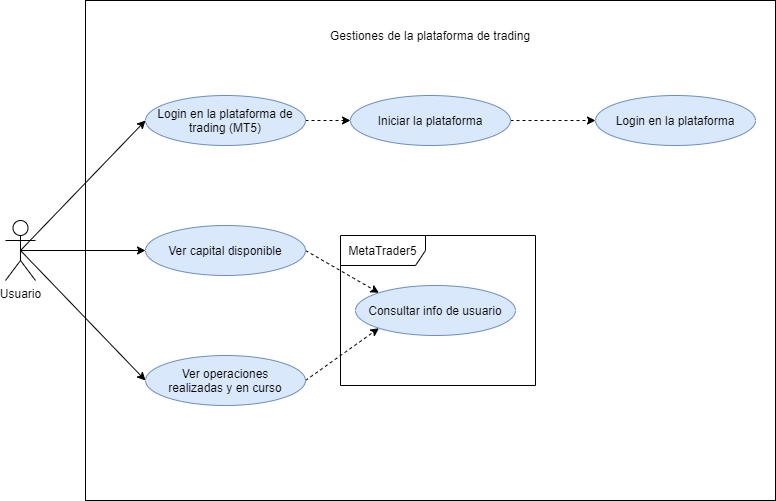
\includegraphics[width=1\textwidth]{imagenes/diagramas_casos_de_uso/CU2-gestiones_MT5.png} 
	\caption{Diagrama de casos de uso referente a la gestión de la plataforma de trading (MT5)}  \label{cu2}
\end{figure}

\subsection{Gestión y visualización de datos de mercados}

El diagrama \ref{cu3} muestra los casos de uso referentes a la gesstión visualización de datos de mercados financieros. Dichos datos serán mostrados mediante un gráfico que muestra precios por medio de velas siguiendo el formato \textit{OHLC}. Para el insertado de dichos datos en el módulo, el usuario seleccionará los parámetros que estime oportunos para la recopilación de los datos históricos. \newline

El usuario podrá ver datos históricos de mercado en un rango de tiempo específico. Este caso de uso interactúa con los datos proporcionados previamente por el usuario. \newline

El usuario de la APP podrá ver datos en tiempo real con un marco de tiempo específico, es decir, con velas generadas cada minuto, cada hora, cada día, etc. Este \textit{CU} usa el módulo de \textit{MT5} para obtener los datos y luego procesa dichos datos para ajustarlos al formato \textit{OHLC}.


\begin{figure}[h] 
	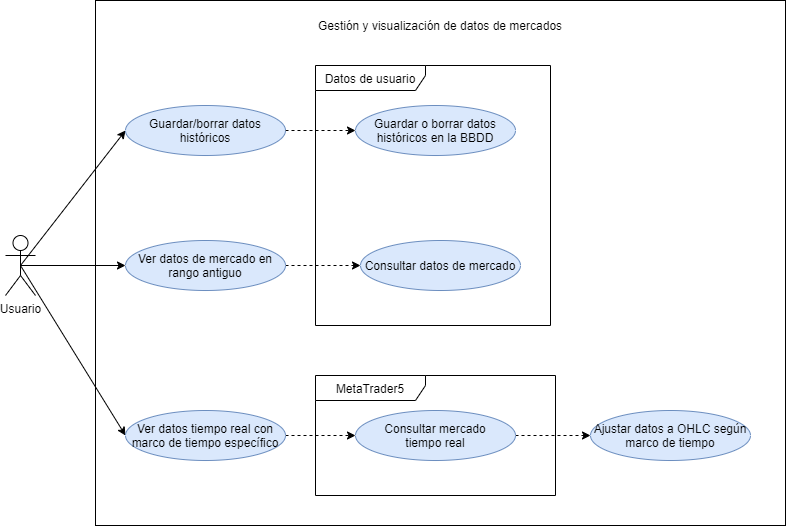
\includegraphics[width=1\textwidth]{imagenes/diagramas_casos_de_uso/CU3-gestion_visualizacion_datos.png} 
	\caption{Diagrama de casos de uso referente a la visualización de datos de mercados financieros} \label{cu3}
\end{figure}


\subsection{Funcionalidades de trading}

Finalmente, el diagrama \ref{cu4} representa los casos de uso referentes al módulo de trading y elección de algoritmos. \newline

El usuario podrá elegir un algoritmo de trading. A la hora de operar, el usuario podrá usar el algoritmo elegido para operar en tiempo real o realizar backtesting. El usuario también podrá operar manualmente, siguiendo su propio análisis en tiempo real, sin algoritmo. \newline

Para los casos de uso de operar manualmente o de forma automática en tiempo real, la APP se conectará al módulo de MT5 para ordenar las operaciones de compra o venta.


\begin{figure}[h] 
	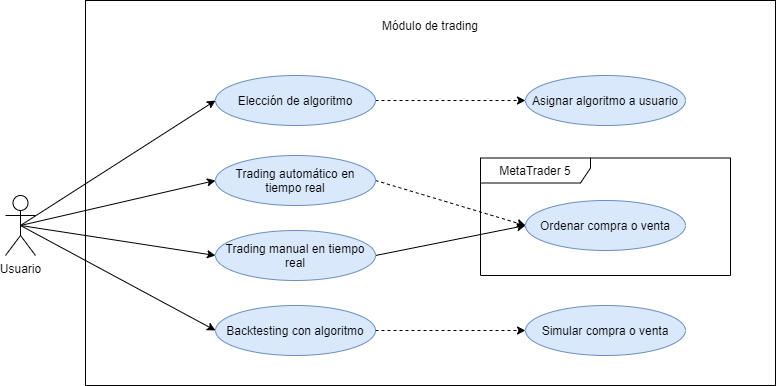
\includegraphics[width=1\textwidth]{imagenes/diagramas_casos_de_uso/CU4-algoritmos.png} 
	\caption{Diagrama de casos de uso referente a las funcionalidades de trading} \label{cu4}
\end{figure}
